\setlength{\footskip}{8mm}

\chapter{Literature Review} 
\label{ch:literature-review}

\textit{Many efficient techniques based on computer vision are available for classification, object detection, and tracking. Here I review existing work that will be useful for the construction of a wrong-way driving system.}

\section{Background Subtraction }
\label{Background Subtraction}
Background subtraction is a commonly-used technique for generating a foreground mask. In background subtraction, a foreground mask is calculated by subtracting the current frame and a background model obtained with a fixed camera. Every object in the background model is considered as part of the background and is to be ignored.

Background modelling has two main steps:\newline
\tab \hspace{8mm}1. Background initialization.\newline
\tab \hspace{8mm}2. Background update, due to possible changes in the scene.\newline
An example is shown in Figure~\ref{fig:background}.

\begin{figure}[t]
  \centering
  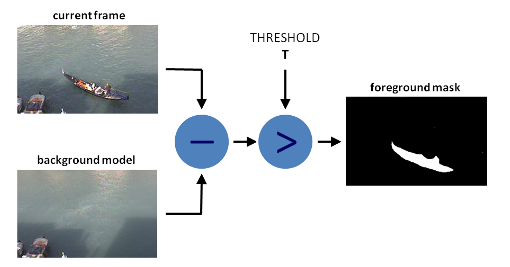
\includegraphics[width=4in]{figures/background.jpg}  
  \caption[background subtraction]{Background subtraction example from \shortciteA{itseez2017theopencv}.}
  \label{fig:background}
\end{figure}

Background subtraction is easy to implement, but it is slow, because background subtraction has to perform its calculation over the whole frame on every frame. Large variance in the background can lead to false negatives, and long-term scene change with a slowly-changing background may not work well.


\section{Classification}
\label{Classification}
Classification is a general technique for determining what something is (when we do not know its type) or determining where something is (when the type of object we are looking for is known).

\subsection{Nearest Neighbor Classification}
The nearest neighbor decision rule assigns a label to an unclassified sample point. The classification model simply contains a set of previously-classified points. The nearest neighbor algorithm will find the nearest item in the training set and return the label of that item. This method is simple to implement and powerful, requiring no training time. This classification method usually has the best accuracy, if the training set is large enough, but it requires too much memory and compute time with a large training set. Also, as shown in Figure~\ref{fig:knn}, if a new data item of class 2 is closer to an item of class 1 than any item of class 2, we would classify the input incorrectly. This can be partly addressed by the K-nearest neighbor method. K-nearest neighbor classification allows the user to specify K, the number of stored items to compare against. The method finds the nearest K items in the training set and returns the label of the majority within that group of items. Thus, in Figure~\ref{fig:knn}, if K = 3, The method will classify the new item as a member of class 2.  

\begin{figure}[t]
  \centering
  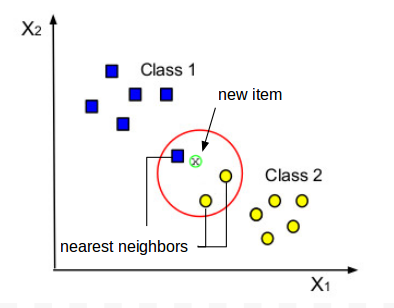
\includegraphics[width=2in]{figures/knn.jpg}   
  \caption[knn]{Example of nearest neighbor classification.}
  \label{fig:knn}
\end{figure}

\subsection{Support Vector Machines}
A support vector machine (SVM) is a feature-based classifier. Suppose we have a set of given data points, each belonging to one of two classes, and the goal is to decide which class a new data point is in SVMs use linear hyperplanes for classification. There are many possible hyperplanes that might classify (separate) the training data correctly. Support vector machines choose the unique hyperplane that provides the largest separation of the training data from the hyperplane, as shown for example in Figure~\ref{fig:svm}. When the training data are not linearly separable, the optimization of the hyperplane is more complicated, but still can be modeled as a constrained quadratic optimization. Support vector machines can induce non-linear classification boundaries due to the \textquotedblleft kernel trick" and do not require a large amount of training data.

\begin{figure}[t]
  \centering
  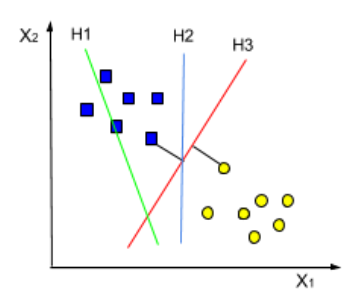
\includegraphics[width=2in]{figures/svm.jpg}   
  \caption[svm]{Example of large margin classification with a linear hyperplane.}
  \label{fig:svm}
\end{figure}


\subsection{Classical Backpropagation Neural Networks}
Backpropagation is a method for training multi-layer neural networks. Usually, a classical neural network would be feature based. Backpropagation over few layers usually has  similar performance to SVMs. The goal of backpropagation is to optimize a set of weights so that the neural network correctly maps arbitrary inputs to a correct output. The optimization algorithm repeats a two-phase cycle, forward propagation and backward weight update. The input is propagated forward through the network, layer by layer, until it reaches the output layer. The output layer is then compared to the desired output using some loss function. The loss is propagated back from the output layer toward the input layer. This method requires  experimentation to tweak hidden layer size and learning time.

\subsection{Convolutional Neural Networks}
The methods described thus far are normally feature based, requiring the data scientist to mathematically specify the set of features to be extracted from the input data. This is necessary when the training set size is small. For images, CNNs offer the benefit of automatically generated features, offering better performance than feature-based methods so long as a sufficient amount of training data is available.

A CNN usually consists of one or more convolutional layers with subsampling steps followed by one or more fully connected layers. The input to a convolutional layer is a $ m \times n \times r $ image, where $m$ is the height, $n$ is the width, and $r$ is the number of channels in the input. The convolutional layer contains $k$ filters or kernels of size $ p \times p \times q $, where $p$ is smaller than the dimension of the image and $q$ can be the same as the number of channels $(r)$ or smaller and may be different for each kernel. The convolutional units share weights across the entire input image patch. Many open source frameworks such as Caffe allow building of CNNs. An example convolution neural network is shown in Figure~\ref{fig:cnn}.

\begin{figure}[t]
  \centering
  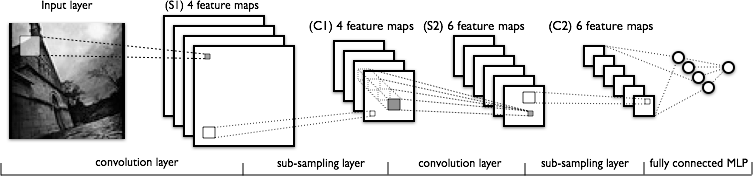
\includegraphics[width=6in]{figures/cnn.jpg}   
  \caption[cnn]{Example convolutional neural network (CNN). Reprinted from \shortciteA{deeplearing}.}
  \label{fig:cnn}
\end{figure}



\section{Object Detection}
\label{Object Detection}
Object detection is a very important part of a computer vision system. Detection helps us find objects in an input image. Most detection methods run a scan window over the image and classify each region as a member or not a member of the object class of interest.



\subsection{Haar Cascades}
Object detection using Haar feature-based cascades is one of the most efficient methods to detect an object in the image. Invented by \shortciteA{viola2001rapid}, this method requires a medium number of input images (positive images and negative images) for training. After training, we use the resulting model to detect objects in other images.

Positive images are images of an object, and negative images are images without that object. In training, we extract the same set of features from both positive and negative images. Each feature is a single value extracted using a fixed binary kernel as shown in Figure~\ref{fig:haar}.

A large set of possible sizes and locations of each kernel are considered, giving a huge number of possible kernels making the training process quite heavy. The trained model might contain a large number of features, which would make it correspondingly inefficient. To increase the efficiency of feature computionation, integral images are used as a memoization method enabling calculation of sums of intensities across rectangular region in constant time regardless of block size. The new problem is then to find which is a good feature, because a good feature should focus on the essential region of the object only. To select features, we use the Adaboost committee building algorithm. The method applies each and every feature to all training images. For each feature, we find the best threshold for classifying the object as positive or negative. Each individual feature in the model is a \textquotedblleft weak classifier" that has same level error of its weighted training set. Different weightings of the training set give different optimal weak classifiers. The best classifier is them a weighted sum of the weak classifiers. Apply all features to each window is not a good idea. This we need Cascade of Classifiers to group the features into different stages of classifiers and apply one-by-one. If a window fails the first stage we do not consider remaining feature on it. The window which passes all stages will be the interest object.

\begin{figure}[t]
  \centering
  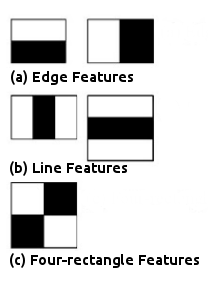
\includegraphics[width=1.5in]{figures/haar.jpg}  
  \caption[Haar kernel ]{Example Haar-like kernels. The sum of the intensities of the pixels in the dark regions is subtracted from those of the light regions. Reprinted from \shortciteA{viola2001rapid}. }
  \label{fig:haar}
\end{figure}



\subsection{Histogram of Oriented Gradients}
Histogram of Oriented Gradients (HOG) \cite{dalal2005histograms} is an object detection technique relying on a holistic descriptor of an image patch. HOG generates a representation of the object is contours. Examples of the same object should produce a descriptor as close as possible to the same descriptor calculated when the object is viewed under different conditions. A support vector machine (SVM) is used to recognize HOG descriptors as representing or not representing the object of interest. To recognize objects at different scales, the image is sub-sampled at multiple sizes. Each of these sub-sampled images is then searched to matches. A sample HOG classifier is shown in Figure~\ref{fig:hog}.

\begin{figure}[t]
  \centering
  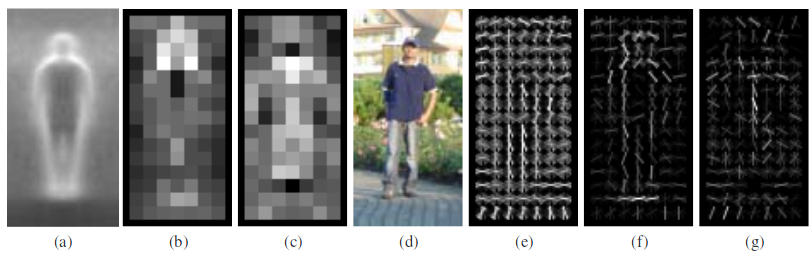
\includegraphics[width=5in]{figures/hog.jpg}  
  \caption[HOG]{HOG classifier. a) The average gradient image over the training examples.  (b) Each “pixel”
shows the maximum positive SVM weight in the block centred on the pixel. (c) Likewise for the negative SVM weights. (d) A test image.
(e) The test image R-HOG descriptor. (f,g) The R-HOG descriptor weighted by respectively the positive and the negative SVM weights. Reprinted from \shortciteA{dalal2005histograms}. }
  \label{fig:hog}
\end{figure}

\subsection{Region-based CNNs}
Region-based CNNs (R-CNNs) \cite{girshick2014rich} combine region proposals with convolutional neural networks (CNNs). When an input image is presented, the system extracts bottom-up region proposals to localize and segment objects. Then it computes features for each proposal by passing each proposal to a convolution neural network. Finally, each region is classified using class-specific linear SVMs. This method yields good results, but it requires a large amount of training data. An overview of the system is shown in Figure~\ref{fig:rcnn}.

For training data, we formed a set of images and boxes that includes all selective search and ground-truth boxes from validation together with up to $N$ ground-truth boxes per class from train. Training data is required for three procedures in R-CNN: (1) CNN find-tuning, (2) detector SVM training, and (3) bounding-box regressor training. Linear SVMs are used to review the definitions briefly, for fine-tuning. 

\begin{figure}[t]
  \centering
  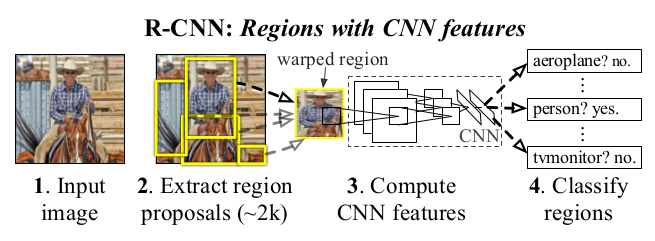
\includegraphics[width=4in]{figures/rcnn.jpg}  
  \caption[R-CNNs]{Object detection system overview. Reprinted from \shortciteA{girshick2014rich}. }
  \label{fig:rcnn}
\end{figure}

\subsection{FAST-RCNNs}
Fast Region-based Convolutional Network method (Fast R-CNN) by \shortciteA{girshick2015fast} builds on R-CNNs to improve training and testing speed while also increasing detection accuracy. Training models in multi-stage pipelines are slow and inelegant. R-CNN is slow because it performs a ConvNet forward pass for each object proposal, without sharing computation. Fast R-CNN takes an input image and multiple regions of interest (RoIs) into a fully convolutional network. Each ROI is pooled into a fixed-size feature map and then mapped to a feature vector by fully connected layers. The network has two output vectors per RoI: softmax probabilities and per-class bounding-box regression offsets. An architecture is shown in Figure~\ref{fig:fastrcnn}. 

\begin{figure}[t]
  \centering
  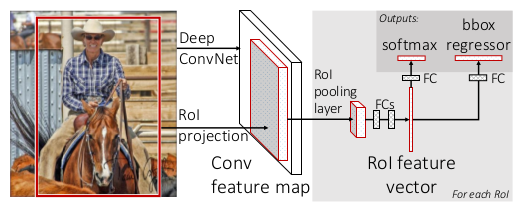
\includegraphics[width=4in]{figures/fastrcnn.jpg}  
  \caption[FAST R-CNNs]{Fast R-CNN architecture. Reprinted from \shortciteA{girshick2015fast}. }
  \label{fig:fastrcnn}
\end{figure}


\section{Optical Flow} 
\label{Optical Flow}
Optical flow (\shortciteA{horn1981determining}) is a technique used for estimating the motion of moving objects in a scene by keeping track of features between consecutive frames. \textquotedblleft Sparse" optical flow methods start by finding strong corners in the image and then calculating the optical flow for the sparse feature set. The most popular and efficient method is the iterative Lucas-Kanade pyramid method.

Optical flow works on two assumptions:\newline
\tab \hspace{8mm}1. The pixel intensities of an object do not change between consecutive frames.\newline
\tab \hspace{8mm}2. Neighbouring pixels have similar motion.

Consider the motion of a pixel $I(x,y,t)$ (where $t$ is time) that is observed in several consecutive frames. If the object moves by a distance $(dx,dy)$ between two frames taking $dt$ time, under the invariant intensity assumption, we have
\[
\begin{array}{lc}
  {\rm } & {I(x,y,t)} = I(x+dx,y+dy,t+dt). \\ \tag{2.1} \label{eq:2.1}
\end{array}
\]
We perform a Taylor series approximation
\[
\begin{array}{lc}
  {\rm } & {I(x+dx,y+dy,t+dt) \approx I(x,y,t) + \frac{\partial I}{\partial x}dx+\frac{\partial I}{\partial y}d y+\frac{\partial I}{\partial t}dt}.\\ 
\end{array}
\]
From equation \eqref{eq:2.1}, since ${I(x,y,t)} = I(x+dx,y+dy,t+dt) = 0$, and dividing by $dt$ we obtain
\[
\begin{array}{lc}
  {\rm } & {\frac{\partial I}{\partial x}\frac{dx}{dt}+\frac{\partial I}{\partial y}\frac{d y}{d t}+\frac{\partial I}{\partial t}\frac{dt}{dt} = 0}.\\ 
\end{array}
\]
\[
\begin{array}{lc}
  {\rm } & {f_xu + f_yv+ f_t }= 0 \\ 
\end{array}
\]
where:
\[
\begin{array}{lc}
  {\rm } & {f_x = \frac{\partial I}{\partial x} \; ; \; f_y = \frac{\partial I}{\partial y} ; \; f_y = \frac{\partial I}{\partial t}}\\ 
\end{array}
\]
\[
\begin{array}{lc}
  {\rm } & {u = \frac{dx}{dt} \; ; \; v = \frac{dy}{dt}.}\\ 
\end{array}
\]
The image gradients are $ f_x $ and $ f_y $. $ f_t $ is a gradient over time. $u$ and $v$ (the pixel motion) are the unknowns. One method to solve this problem is Lucas-Kanade.

According to the assumption, neighbouring pixels must have similar motion. Lucas-Kanade therefore takes a 3 $ \times $ 3 patch around each point. These nine pixels are all assumed to have the same motion, so we find  $ (f_x,f_y,f_t) $ for these nine points. We obtain have nine equations in the two unknown variables. The least-squares solution for this is shows below.
\[
\begin{array}{lc}
  {\rm } & {  \begin{bmatrix} u \\ v \end{bmatrix} = \begin{bmatrix} \sum_{i}{f_{x_i}}^2 & \sum_{i}{f_{x_i} f_{y_i} } \\ \sum_{i}{f_{x_i} f_{y_i}} & \sum_{i}{f_{y_i}}^2 \end{bmatrix}^{-1} \begin{bmatrix} - \sum_{i}{f_{x_i} f_{t_i}} \\ - \sum_{i}{f_{y_i} f_{t_i}} \end{bmatrix}  }.\\ 
\end{array}
\]
Large motions will be difficult to identify with this method. Hence, Lucas-Kanade is applied in a pyramid. At higher levels of the pyramid, small motions are ignored, and large motions of large regions become small motions of small regions that can be identified using the same method as above.

\section{Traffic Flow Direction Learning}
\shortciteA{monteiro2007wrongway} present work on a system whose basic idea is to get the correct direction of motion of vehicles in different lanes is during a learning period when it is assumed that traffic is flowing in the correct direction. Hence, the system learns the correct direction for each point in the scene. The authors propose a learning method that analyzes many frames. A Gaussian mixture model is learned for each block in the image by analysis of vehicles' movement over time. This method is good; it is able to detect vehicles circulating on the wrong side of the road, and it runs in real-time. But this method may have errors in identifying objects and may not work well on more crowded scenes. Learning process has shown in Figure~\ref{fig:learning}/
 

\begin{figure}[h]
  \centering
  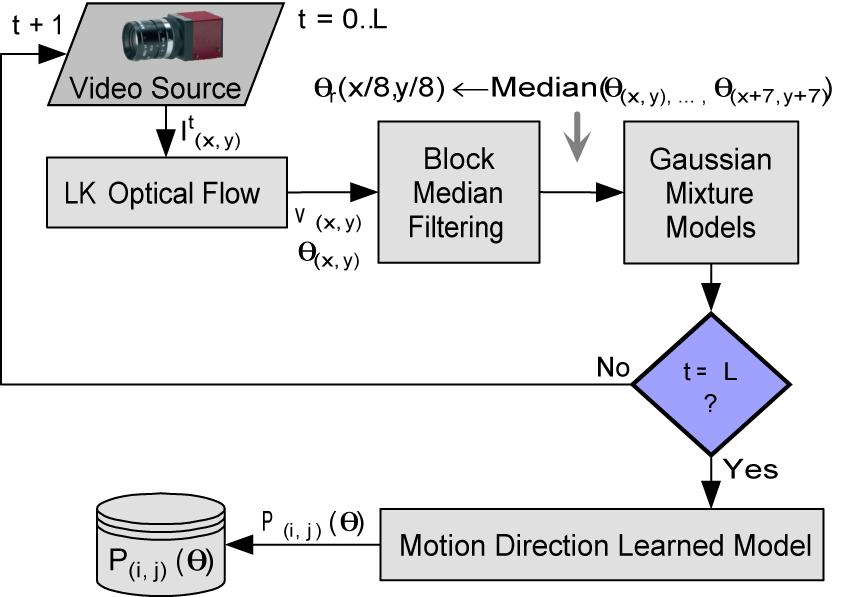
\includegraphics[width=3in]{figures/learning.jpg}  
  \caption[Learning flow chart]{Flow chart of the traffic flow direction learning process. Reprinted from  \shortciteA{monteiro2007wrongway}. }
  \label{fig:learning}
\end{figure}



\section{Object Tracking}
\label{Tracking}
Object tracking has been a problem for research for many years. It is still not a solved problem, but there are many object trackers. Object trackers usually need some initialization step, which can be provided manually or automatically using an object detector.

\subsection{CAMSHIFT}
CAMSHIFT is a practical application of the meanshift method to tracking of an object using a color histrogram. The basis idea of meanshift is a set of points that fit with a small window. A small window should move to the area of maximum number of points. But the problem of meanshift is a size of window is fixed. Camshift trys to solve this problem by adaption the window size and rotation of the target. It updates the size of window as, $ s = 2 \sqrt{\frac{M_{00}}{256}} $ when $s$ is size of window, $M_{00}$ is a zero order moment. Camshift also calculates the orientation of the best-fitting ellipse for the object. Then it applied meanshift with new scaled search window and previous window location. The method keeps executing this process until a threshold is reached.

\subsection{CAMSHIFT}

\FloatBarrier

